\documentclass[english,11pt]{beamer}

\DeclareMathOperator{\Cov}{Cov}
\DeclareMathOperator{\Var}{Var}
\DeclareMathOperator{\E}{\mathbb{E}}
\DeclareMathOperator{\Proba}{\mathbb{P}}

\newcommand{\Covb}[2]{\ensuremath{\Cov\!\left[#1,#2\right]}}
\newcommand{\Eb}[1]{\ensuremath{\E\!\left[#1\right]}}
\newcommand{\Pb}[1]{\ensuremath{\Proba\!\left[#1\right]}}
\newcommand{\Varb}[1]{\ensuremath{\Var\!\left[#1\right]}}

% norm
\newcommand{\norm}[1]{\| #1 \|}

\newcommand{\indep}{\rotatebox[origin=c]{90}{$\models$}}





\usepackage{mathptmx,amsmath,amssymb,graphicx,bibentry,bbm,babel,ragged2e}

\makeatletter

\newcommand{\noun}[1]{\textsc{#1}}
\newcommand{\jitem}[1]{\item \begin{justify} #1 \end{justify} \vfill{}}
\newcommand{\sframe}[2]{\frame{\frametitle{#1} #2}}

\newenvironment{centercolumns}{\begin{columns}[c]}{\end{columns}}
%\newenvironment{jitem}{\begin{justify}\begin{itemize}}{\end{itemize}\end{justify}}

\usetheme{Warsaw}
\setbeamertemplate{footline}[text line]{}
\setbeamercolor{structure}{fg=purple!50!blue, bg=purple!50!blue}

\setbeamersize{text margin left=15pt,text margin right=15pt}

\setbeamercovered{transparent}


\@ifundefined{showcaptionsetup}{}{%
 \PassOptionsToPackage{caption=false}{subfig}}
\usepackage{subfig}

\usepackage[utf8]{inputenc}
\usepackage[T1]{fontenc}

\usepackage{multirow}


\makeatother

\begin{document}





\title{Multiscalar models for systems of cities}

\author{J.~Raimbault$^{1,2,3,4,\ast}$\\
\texttt{$\ast$ juste.raimbault@ign.fr}
}


\institute{$^{1}$ LASTIG, IGN-ENSG\\
$^{2}$CASA, UCL\\
$^{3}$UPS CNRS 3611 ISC-PIF\\
$^{4}$UMR CNRS 8504 G{\'e}ographie-cit{\'e}s
}


\date{ECTQG 2023\\\smallskip
September 15th 2023
}

\frame{\maketitle}



\sframe{An evolutionary theory for urban systems}{

% Simulation models for the dynamics of systems of cities have been developed to capture salient stylised facts of such systems and understand underlying processes (Pumain & Reuillon, 2017). These agent-based models simulate the interactions between cities at the macroscopic scale, focusing on different dimensions such as innovation or economic exchanges. They correspond to the highest level of the multiscalar ontology described by Pumain (2011) for urban systems.



\begin{center}
	\begin{columns}
	\begin{column}{0.45\linewidth}
	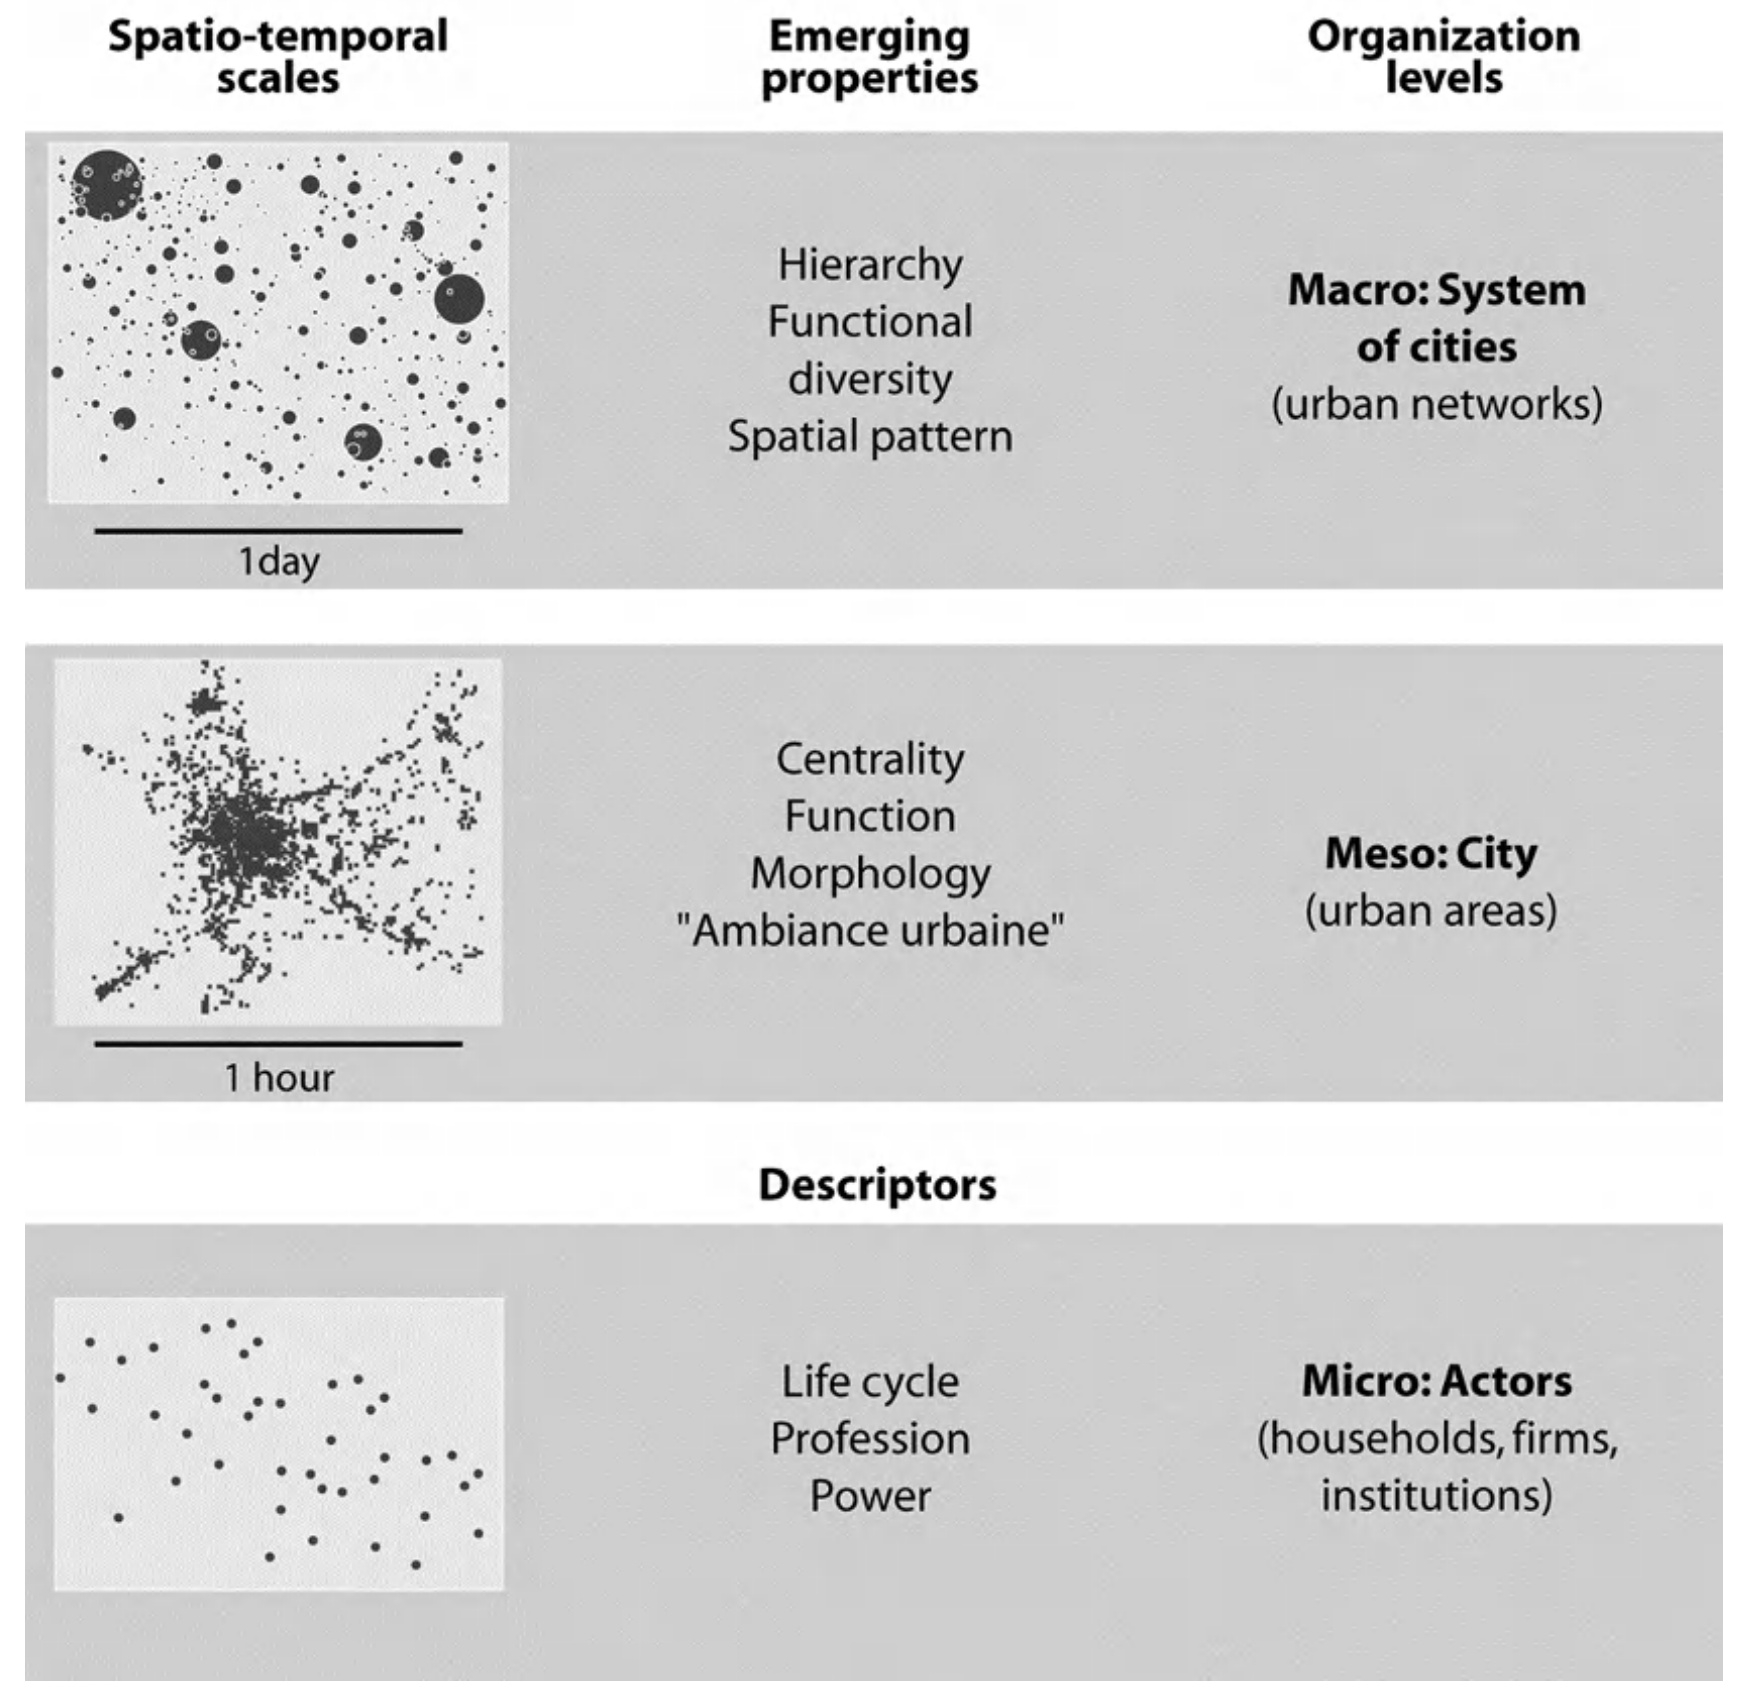
\includegraphics[width=\textwidth]{../../2020/ALife2020/figures/evoltheory_scales.png}
	\end{column}
	\begin{column}{0.22\linewidth}
	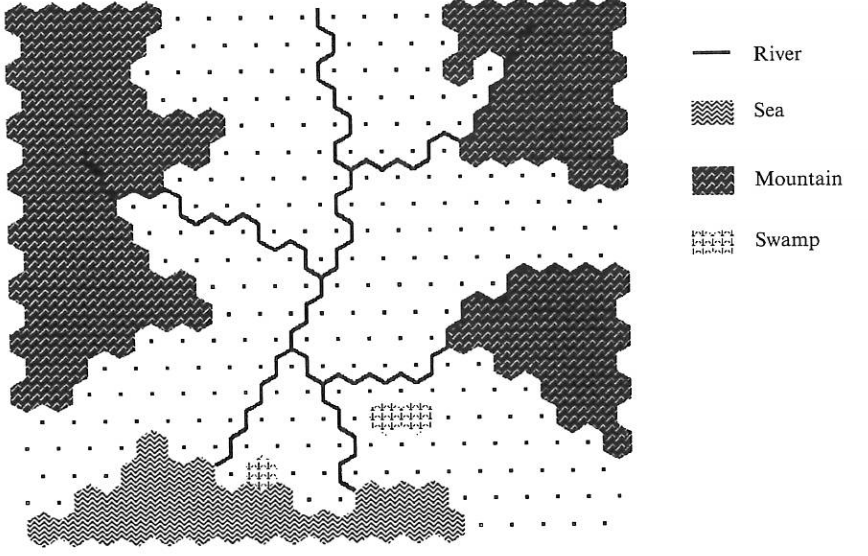
\includegraphics[width=\textwidth]{../../2020/ALife2020/figures/simpop1.png}\\\medskip
	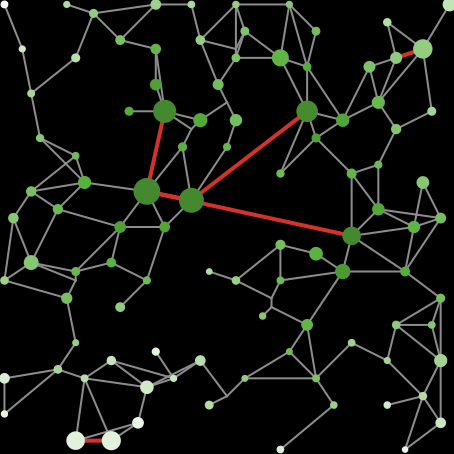
\includegraphics[width=\textwidth]{../../2020/ALife2020/figures/setup_synth_1_tick100.png}
	\end{column}
	\end{columns}
\end{center}

\footnotesize
\textit{An evolutionary urban theory considering cities as systems within systems of cities \cite{pumain2018evolutionary}; Simpop 1 model \cite{sanders1997simpop}; SimpopNet model \cite{schmitt2014modelisation}}



}


\sframe{Multi-modeling urban systems dynamics}{

% sdg tradeoffs, multiobj ersa2022



}



\sframe{Hybrid models}{

% Lutecia and physical network: "semi-multiscale"

}


\sframe{Towards multiscale models}{

% In order to address open issues related to multi-level governance of territorial sustainable transitions, models simulating simultaneously multiple scales are however needed (Rozenblat & Pumain, 2018).

% contribution




}

\sframe{Urban morphology and inter-city interactions}{

% This contribution synthesises recent lessons learnt from the construction and exploration of such strongly coupled multi-scalar models. The first model couples a macroscopic population dynamics model with local urban morphogenesis models within each city (Raimbault, 2021),

% broad description of morph-intgib model: cit ccs19 and preprint

}

\sframe{Model exploration}{

% salient results for urbmorph-intgib

}



\sframe{Multi-scale innovation dynamics}{

% while the second one simulates the diffusion of innovation between urban areas and its impact on urban growth at the macroscopic scale, and innovation cluster dynamics within each area (Raimbault & Pumain, 2023).

}


\sframe{Model exploration}{

}


\sframe{Common aspects from simulation results}{

% First simulation results show that strong emergence appears in a significant number of regimes for the innovation model, and that contradictory objectives across scales can be simultaneously optimised using multi-objective genetic algorithms for both models.


}




\sframe{Teaching 1: ontologies and feedbacks}{


% A few pitfalls have been identified while theoretically constructing the models and empirically exploring their parameter space using advanced model validation techniques with the OpenMOLE software (Reuillon et al., 2013): (i) to obtain a strong coupling between scales, and thus effective multiscalar dynamics rather than fixed effects at the meso scale only for example, both top-down and bottom-up feedbacks have to be included explicitly, and corresponding ontologies and processes must be identified; 


}


\sframe{Teaching 2: consistent data parametrisation}{

%ii) the parametrisation or calibration with empirical data is significantly more cumbersome than with single level models, and synthetic systems are a first alternative to explore model behaviour; 

}


\sframe{Teaching 3: stochasticity}{

% (iii) the convergence of model indicators regarding stochasticity seems more difficult to obtain, possibly due to non-linear noise propagation between scales; 

% TODO histogram/distib for illustrated indicators for the innovation model?

}


\sframe{Teaching 4: quantifying strong emergence}{

% (iv) a crucial aspect remains to quantify the strength of emergence, such that these approaches are not a superfluous complication of simpler dynamics at a single scale – the indicators introduced by (Rosas et al., 2020) are good candidates for such measures but remain to be tested systematically on geosimulation models.



}





\sframe{Discussion}{


% \textbf{Main results:}


\justify

$\rightarrow$ 
			
\bigskip
				
$\rightarrow$ 

\bigskip

%\textbf{Conclusion: } 

}









%%%%%%%%%%%%%%%%%%%%%
\begin{frame}[allowframebreaks]
\frametitle{References}
\bibliographystyle{apalike}
\bibliography{biblio}
\end{frame}
%%%%%%%%%%%%%%%%%%%%%%%%%%%%




\end{document}









